% Fig. 2: Data and training pipeline (surrogate pretraining, then sparse CGYRO correction).
% Built from the scientific-schematics ML pipeline template.
\documentclass[tikz,border=6pt]{standalone}
\usepackage[scaled]{helvet}\renewcommand{\familydefault}{\sfdefault}
\usepackage{amsmath}
\usepackage[italic]{mathastext}
\usetikzlibrary{positioning,arrows.meta,shapes.geometric,fit,backgrounds,calc}

\definecolor{oiOrange}{HTML}{E69F00}\definecolor{oiSky}{HTML}{56B4E9}
\definecolor{oiGreen}{HTML}{009E73}\definecolor{oiYellow}{HTML}{F0E442}
\definecolor{oiBlue}{HTML}{0072B2}\definecolor{oiVermil}{HTML}{D55E00}
\definecolor{oiPurple}{HTML}{CC79A7}

\tikzset{
  base/.style={draw, align=center, font=\footnotesize, line width=0.6pt,
               text width=22mm, minimum height=13mm, inner sep=2pt},
  proc/.style={base, rounded corners=2pt, fill=oiSky!22, draw=oiBlue},
  store/.style={base, cylinder, shape border rotate=90, aspect=0.18,
                text width=19mm, fill=oiOrange!22, draw=oiOrange!80!black},
  model/.style={base, rounded corners=6pt, fill=oiGreen!22, draw=oiGreen!80!black},
  mon/.style={base, rounded corners=2pt, fill=oiPurple!22, draw=oiPurple!80!black},
  arr/.style={-{Stealth[length=2.2mm]}, line width=0.7pt, draw=black!80},
  lbl/.style={font=\scriptsize, fill=white, inner sep=1pt},
  lane/.style={draw=black!25, fill=black!3, rounded corners=4pt, inner sep=4mm},
  lanetitle/.style={font=\small\bfseries, text=black!70, anchor=north west},
}

% ---- legend swatches: small, vertically centred copies of each box style ----
% \boxswatch[corner radius]{fill/draw options}
\newcommand{\boxswatch}[2][1.5pt]{\tikz[baseline=-0.6ex]\draw[line width=0.6pt, rounded corners=#1, #2] (0,-1.4mm) rectangle (5.5mm,1.4mm);}
\newcommand{\cylswatch}{\tikz[baseline=-0.6ex]{%
  \draw[line width=0.6pt, fill=oiOrange!22, draw=oiOrange!80!black]
       (0,1.0mm) -- (0,-1.0mm) arc[start angle=180, end angle=360, x radius=2mm, y radius=0.55mm] -- (4mm,1.0mm);
  \draw[line width=0.6pt, fill=oiOrange!22, draw=oiOrange!80!black] (2mm,1.0mm) ellipse[x radius=2mm, y radius=0.55mm];}}
\newcommand{\arrswatch}[1]{\tikz[baseline=-0.6ex]\draw[#1] (0,0) -- (7mm,0);}
\newcommand{\gap}{\hspace{5mm}}

\begin{document}
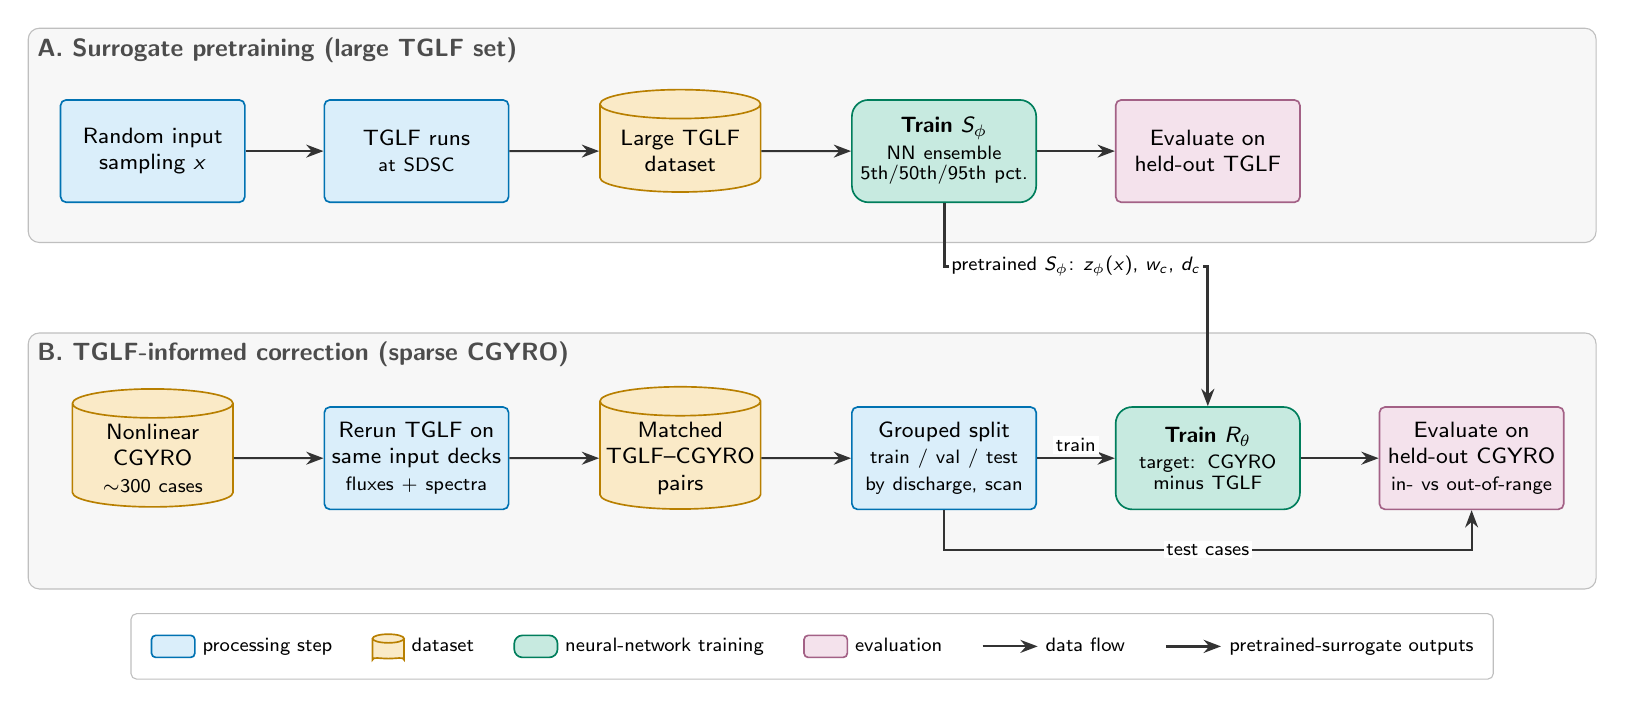
\begin{tikzpicture}
\def\dx{3.35}

% ---------------- Stage A: surrogate pretraining ----------------
\node[proc]  (samp)  at (0*\dx,0) {Random input\\sampling $x$};
\node[proc]  (tglfA) at (1*\dx,0) {TGLF runs\\{\scriptsize at SDSC}};
\node[store] (bulk)  at (2*\dx,0) {Large TGLF\\dataset};
\node[model] (trS)   at (3*\dx,0) {\textbf{Train} $S_\phi$\\{\scriptsize NN ensemble}\\[-2pt]{\scriptsize 5th/50th/95th pct.}};
\node[mon]   (evS)   at (4*\dx,0) {Evaluate on\\held-out TGLF};

\draw[arr] (samp) -- (tglfA);
\draw[arr] (tglfA) -- (bulk);
\draw[arr] (bulk) -- (trS);
\draw[arr] (trS) -- (evS);

% ---------------- Stage B: sparse CGYRO correction ----------------
\def\yB{-3.9}
\node[store] (cg)    at (0*\dx,\yB) {Nonlinear\\CGYRO\\{\scriptsize $\sim$300 cases}};
\node[proc]  (tglfB) at (1*\dx,\yB) {Rerun TGLF on\\same input decks\\{\scriptsize fluxes + spectra}};
\node[store] (pairs) at (2*\dx,\yB) {Matched\\TGLF--CGYRO\\pairs};
\node[proc]  (split) at (3*\dx,\yB) {Grouped split\\{\scriptsize train / val / test}\\{\scriptsize by discharge, scan}};
\node[model] (trR)   at (4*\dx,\yB) {\textbf{Train} $R_\theta$\\{\scriptsize target: CGYRO}\\[-2pt]{\scriptsize minus TGLF}};
\node[mon]   (evR)   at (5*\dx,\yB) {Evaluate on\\held-out CGYRO\\{\scriptsize in- vs out-of-range}};

\draw[arr] (cg) -- (tglfB);
\draw[arr] (tglfB) -- (pairs);
\draw[arr] (pairs) -- (split);
\draw[arr] (split) -- node[lbl, above=1pt] {train} (trR);
\draw[arr] (trR) -- (evR);
\draw[arr] (split.south) -- ++(0,-5mm) -| node[lbl, pos=0.25] {test cases} (evR.south);

% ---------------- pretrained surrogate feeds the correction ----------------
\draw[arr, line width=1.1pt] (trS.south) -- ++(0,-8mm) -| node[lbl, pos=0.25, align=center]
     {pretrained $S_\phi$: $z_\phi(x)$, $w_c$, $d_c$} (trR.north);

% ---------------- Lanes ----------------
\begin{scope}[on background layer]
  \node[lane, fit=(samp)(evS)(evR.east |- samp), inner ysep=7mm, yshift=2mm] (L1) {};
  \node[lanetitle] at (L1.north west) {A.\ Surrogate pretraining (large TGLF set)};
  \coordinate (bL) at ($(samp.west |- split.south)+(0,-7mm)$);
  \node[lane, fit=(cg)(evR)(bL)(samp.west |- cg.north), inner ysep=5mm, yshift=2mm] (L2) {};
  \node[lanetitle] at (L2.north west) {B.\ TGLF-informed correction (sparse CGYRO)};
\end{scope}

% ---------------- Legend ----------------
\node[anchor=north, font=\scriptsize, align=left, draw=black!25, rounded corners=2pt, inner sep=2.5mm]
     at ($(current bounding box.south)+(0,-3mm)$) {%
  \boxswatch{fill=oiSky!22, draw=oiBlue}\ processing step\gap
  \cylswatch\ dataset\gap
  \boxswatch[3pt]{fill=oiGreen!22, draw=oiGreen!80!black}\ neural-network training\gap
  \boxswatch{fill=oiPurple!22, draw=oiPurple!80!black}\ evaluation\gap
  \arrswatch{arr}\ data flow\gap
  \arrswatch{arr, line width=1.1pt}\ pretrained-surrogate outputs};

\end{tikzpicture}
\end{document}
